\documentclass[aspectratio=169]{beamer}
\usetheme{Madrid}
\usepackage[utf8]{inputenc}
\usepackage[T1]{fontenc}
\usepackage{tikz}
\usepackage{amssymb}
\usepackage{graphicx}
\setbeamertemplate{navigation symbols}{}
\setbeamercolor{title}{fg=white,bg=red!75!black}
\setbeamercolor{frametitle}{fg=white,bg=red!75!black}
\setbeamercolor{block title}{bg=red!75!black!20,fg=black}
\setbeamercolor{block body}{bg=red!75!black!8,fg=black}
\setbeamercolor{item}{fg=red!75!black}
\setbeamercolor{itemize item}{fg=red!75!black}
\setbeamertemplate{itemize item}[triangle]

\title{Security Lab — Spot the Scam}
\subtitle{Real online safety: scam messages, stranger danger, and phishing links}
\author{ByteForge --- Grade 7 --- Game Maker}
\date{}

\begin{document}

\begin{frame}
    \titlepage
\end{frame}

\begin{frame}{Today's Plan}
    \begin{itemize}
        \item Too Good to Be True
        \item Strangers Never Need Your Address
        \item The "Free Skins" Trap
        \item[$\bigstar$] BOSS --- Build a Scam Checker
    \end{itemize}
\end{frame}

\begin{frame}{A surprise free prize is the \#1 real scam sign}
    \large
    \begin{itemize}
        \item Real companies do not give away expensive prizes to random strangers who never entered anything
        \item The free prize is the bait, not a real gift. \texttt{isScam} set to true, checked by a real if/else, is exactly how a real spam filter works underneath.
    \end{itemize}
\end{frame}


\begin{frame}{Friendly in chat does not mean safe in real life}
    \large
    \begin{itemize}
        \item Someone you only know from an online game has NO real reason to need your address, school, or real name
        \item Asking for these is a genuine red flag, even if they seem friendly. There is no way to verify who someone really is over game chat.
    \end{itemize}
\end{frame}


\begin{frame}{A "free skins" site exists to steal your password}
    \large
    \begin{itemize}
        \item Sites promising free skins in exchange for "logging in with your real account" are built to capture your actual password the instant you type it
        \item A genuinely common real scam aimed specifically at gamers. Only the game's own official site or app is ever safe.
    \end{itemize}
\end{frame}


\begin{frame}{BOSS — combining every red flag into one real check}
    \large
    \begin{itemize}
        \item A stranger AND a free offer together is a stronger warning than either alone
        \item Combining two variables in one if/else genuinely mirrors how real scam/spam filters weigh several signals together, not just one.
    \end{itemize}
\end{frame}

\begin{frame}{Real-World Examples}
    \large
    \begin{itemize}
        \item A message promising a free prize "just for clicking" uses the exact same bait-and-hook pattern as a real phishing email
        \item Designed to get a click before you think. A fake "free V-Bucks generator" asking you to log in first is a genuine, extremely common real scam, not a hypothetical one.
    \end{itemize}
\end{frame}


\begin{frame}{Image}
    \begin{center}
    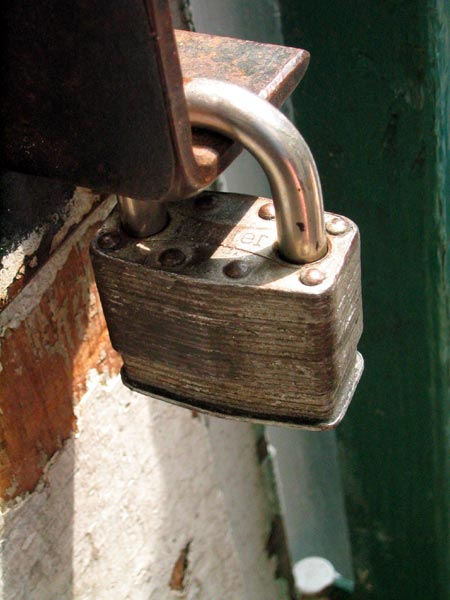
\includegraphics[width=0.5\textwidth]{images/padlock.jpg}

    \large What a real password is actually protecting --- exactly what a fake "free skins" site is trying to steal.

    \small Padlock — Alyson Hurt, CC BY 2.0, via Wikimedia Commons
    \end{center}
\end{frame}

\begin{frame}{Let Them Discover (1/2)}
    \Large
    Has anyone you know ever gotten a message online promising something free in exchange for personal info or a login? What made it feel suspicious (or NOT feel suspicious at first)?
\end{frame}


\begin{frame}{Let Them Discover (2/2)}
    \Large
    Look at a real login page for a game or app you use. What would be different about a FAKE version of that same page trying to steal your password?
\end{frame}

\begin{frame}{Your Turn}
    \Large
    Open the student map, find \textbf{Security Lab — Spot the Scam}, and work through it
    hands-on --- everything you just saw, they now do themselves.
\end{frame}

\end{document}
